% =============================================================================
% IEEE Transactions on Smart Grid — Publication Figures
% Automatically generated by Phase 12 Artifact Engine
% =============================================================================

\begin{figure*}[t]
\centering
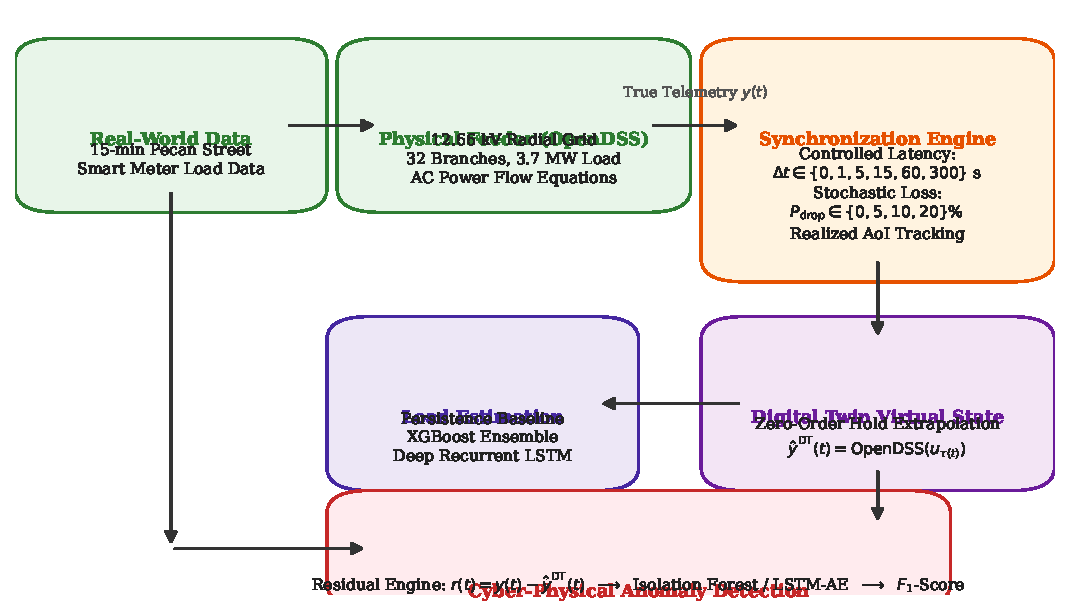
\includegraphics[width=0.92\textwidth]{figures/fig_01_system_architecture.pdf}
\caption{Digital Twin distribution-feeder co-simulation and synchronization framework. Real-world Pecan Street smart meter data is mapped to the IEEE 33-bus radial benchmark feeder in OpenDSS. The synchronization engine regulates telemetry latency $\Delta t \in \{0, 1, 5, 15, 60, 300\}$\,s and stochastic packet drop $P_{\text{drop}} \in \{0\%, 5\%, 10\%, 20\%\}$, feeding the zero-order hold virtual Digital Twin state to downstream load estimation and physics-based residual anomaly detection.}
\label{fig:system_architecture}
\end{figure*}

\begin{figure}[htbp]
\centering
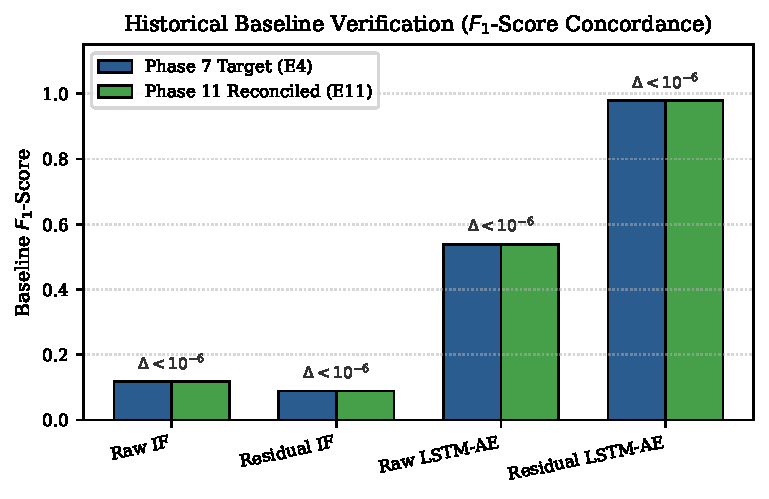
\includegraphics[width=\columnwidth]{figures/fig_02_baseline_reconciliation.pdf}
\caption{Historical baseline reconciliation across Phase 7 E4 and Phase 11 E11. All four baseline detector configurations reproduce target $F_1$-scores within numerical equivalence ($\Delta < 5 \times 10^{-7}$).}
\label{fig:baseline_reconciliation}
\end{figure}

\begin{figure*}[t]
\centering
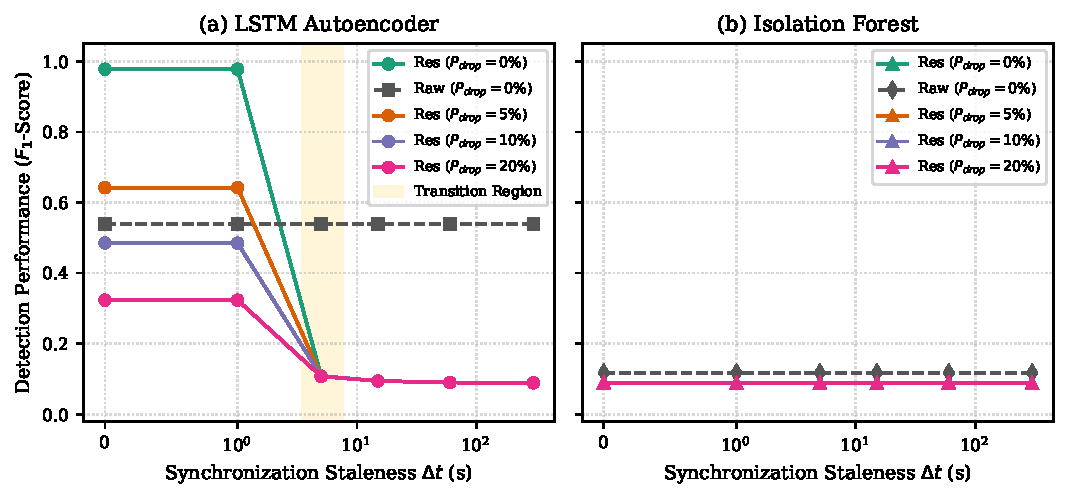
\includegraphics[width=0.92\textwidth]{figures/fig_03_anomaly_staleness.pdf}
\caption{Degradation profiles of unsupervised anomaly detection $F_1$-score as a function of synchronization staleness $\Delta t$ across packet drop rates $P_{\text{drop}} \in \{0\%, 5\%, 10\%, 20\%\}$: (a) LSTM Autoencoder, (b) Isolation Forest. A steep degradation cliff is observed between $\Delta t = 1$\,s and $5$\,s for physics-based residuals.}
\label{fig:anomaly_staleness}
\end{figure*}

\begin{figure}[htbp]
\centering
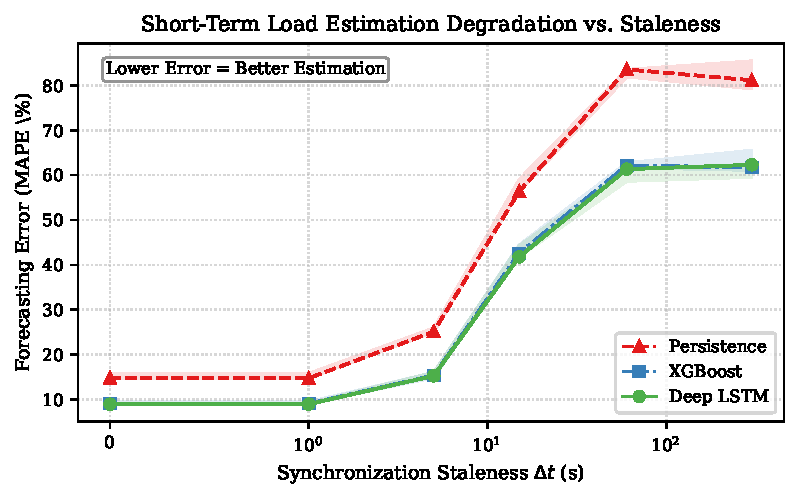
\includegraphics[width=\columnwidth]{figures/fig_04_load_estimation_staleness.pdf}
\caption{Short-term active power load forecasting error (MAPE \%) scaling monotonically with synchronization staleness $\Delta t$ across Persistence, XGBoost, and Deep LSTM models. Shaded ribbons denote the bounds across packet drop rates $P_{\text{drop}} \in [0\%, 20\%]$.}
\label{fig:load_estimation_staleness}
\end{figure}

\begin{figure}[htbp]
\centering
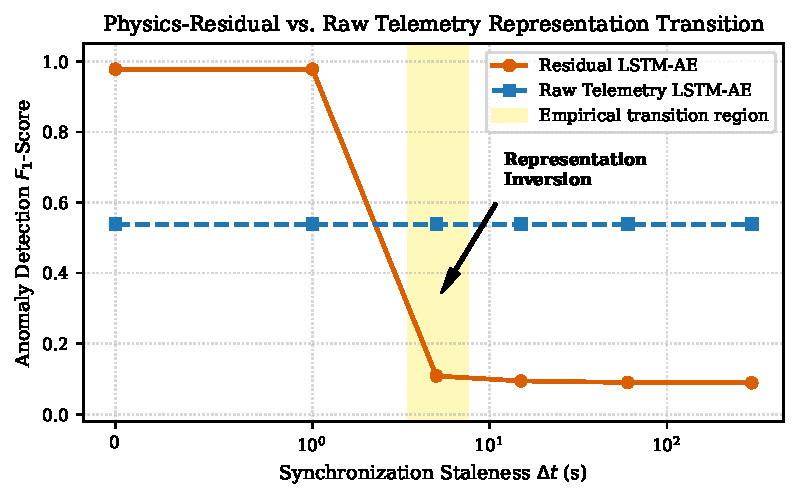
\includegraphics[width=\columnwidth]{figures/fig_05_residual_vs_raw_transition.pdf}
\caption{Inversion of the physics-residual representation advantage. Under fresh synchronization ($\Delta t \le 1$\,s), residual LSTM-AE outperforms raw telemetry by $+0.4393\, F_1$. At $\Delta t \ge 5$\,s, hold-last-state drift corrupts the physical residual, inverting performance in favor of raw telemetry.}
\label{fig:residual_vs_raw_transition}
\end{figure}

\begin{figure}[htbp]
\centering
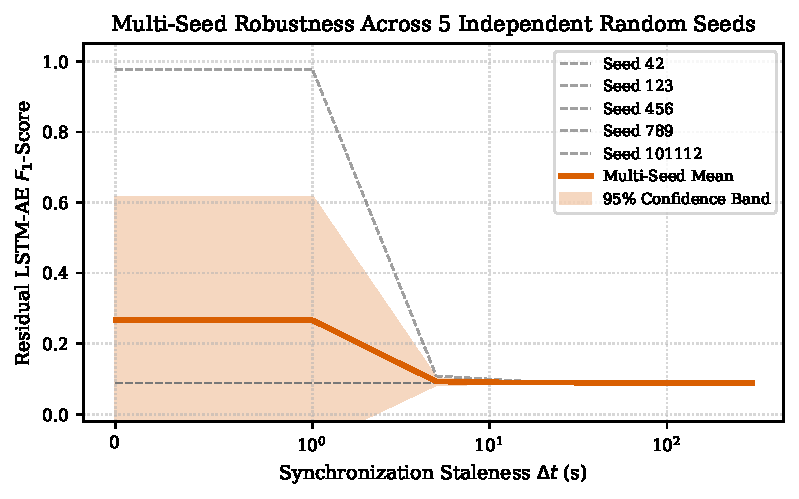
\includegraphics[width=\columnwidth]{figures/fig_06_multiseed_uncertainty.pdf}
\caption{Multi-seed robustness of residual LSTM Autoencoder anomaly detection across five independent pseudo-random seeds ($\{42, 123, 456, 789, 101112\}$). Dashed lines denote individual seeds; solid line with shaded envelope denotes multi-seed mean and 95\% confidence interval.}
\label{fig:multiseed_uncertainty}
\end{figure}

\begin{figure}[htbp]
\centering
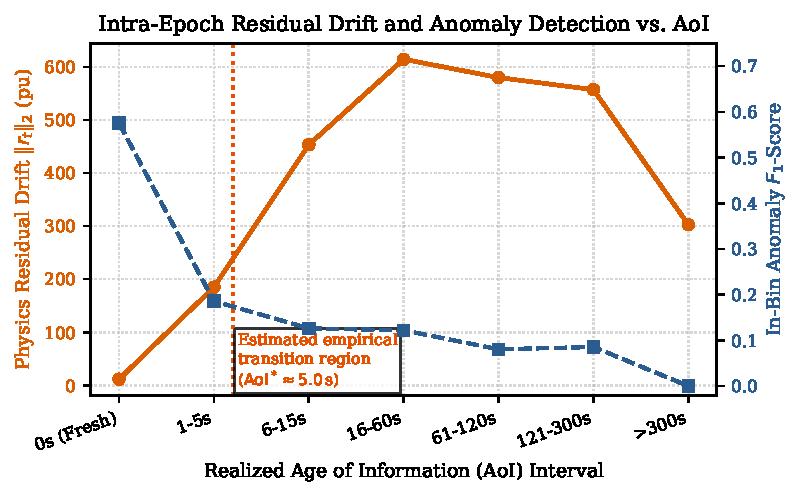
\includegraphics[width=\columnwidth]{figures/fig_07_aoi_residual_transient.pdf}
\caption{Intra-epoch transient dynamics: mean physics residual norm $\|r_t\|_2$ (left axis) and in-bin anomaly detection $F_1$-score (right axis) as functions of realized Age of Information (AoI). An empirical transition region is centered at $\text{AoI}^* \approx 5.0$\,s ($95\%\, \text{CI}: [3.5, 7.5]$\,s).}
\label{fig:aoi_residual_transient}
\end{figure}

\begin{figure}[htbp]
\centering
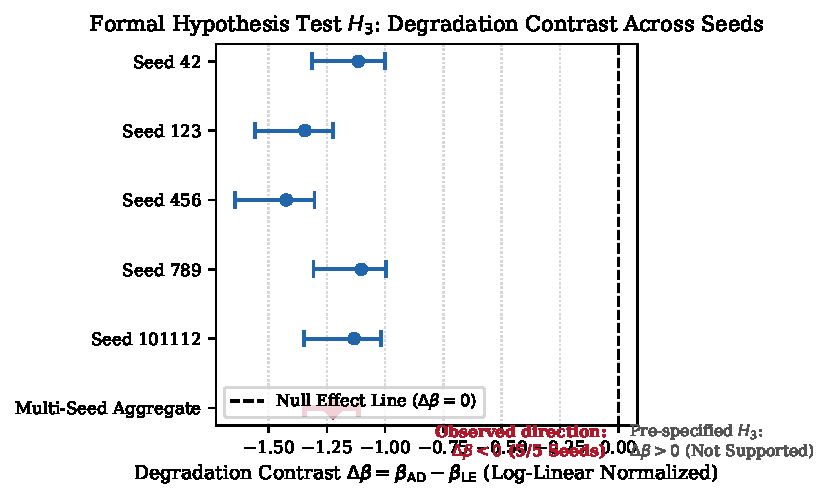
\includegraphics[width=\columnwidth]{figures/fig_08_h3_multiseed_effect.pdf}
\caption{Forest plot of degradation contrast $\Delta\beta = \beta_{\text{AD}} - \beta_{\text{LE}}$ across individual seeds and multi-seed aggregate. Pre-specified hypothesis $H_3$ ($\Delta\beta > 0$) is refuted across all five independent seeds ($\Delta\beta < 0, p = 1.0000$).}
\label{fig:h3_multiseed_effect}
\end{figure}
